% !TEX TS-program = pdflatex
% !TEX encoding = UTF-8 Unicode

\documentclass[handout,svgnames]{beamer}
%\documentclass{beamer}

%\usepackage{pgfpages} %for {show notes on second screen option}

\mode<presentation>
{
  %\usetheme{Rochester} %pretty plain, no footer and progress
  %\usetheme{Marburg}   %sidebar with all (sub)sections
  %\usetheme{Madrid}	%footer with author, title, date and frame number, 
  %\usetheme{Luebeck}		%big header with all sections, footer with author and title
  \usetheme{Frankfurt}  %favorite for now %header with progress
  %\usetheme{Dresden}	%header with progress, 2 footers for author an title
  %\usetheme{Copenhagen}	%big header with all sections, footer with author and title
  %\usetheme{Berlin}		%header with progress, 2 footers for author an title
  %\usetheme{Warsaw}		%big header with all sections, footer with author and title
%\setbeamercolor*{palette primary}{use=structure,fg=white,bg=DarkGreen}
\useinnertheme{circles} %bullet points look nice to me that way (especially numbered ones)

\setbeamertemplate{footline}
{
  \leavevmode%
  \hbox{%
  \begin{beamercolorbox}[wd=.45\paperwidth,ht=2.25ex,dp=1ex,center]{author in head/foot}%
    \usebeamerfont{author in head/foot}\insertshortauthor
  \end{beamercolorbox}%
  \begin{beamercolorbox}[wd=.45\paperwidth,ht=2.25ex,dp=1ex,center]{title in head/foot}%
    \usebeamerfont{title in head/foot}\insertshorttitle\hspace*{3em}
  \end{beamercolorbox}%
  \begin{beamercolorbox}[wd=.1\paperwidth,ht=2.25ex,dp=1ex,center]{author in head/foot}%
    \insertframenumber{} / \inserttotalframenumber\hspace*{1ex}  
  \end{beamercolorbox}}%

  \vskip0pt%
}

  %\setbeamercovered{transparent}
  % or whatever (possibly just delete it)

\setbeamertemplate{navigation symbols}{}%remove navigation symbols
%\setbeameroption{show notes on second screen}
}

\usepackage[ngerman]{babel}
\usepackage[utf8x]{inputenc}
\usepackage[T1]{fontenc}
\usepackage{eurosym} %for euro symbol via \euro

\usepackage{graphicx}
\usepackage{wrapfig}

%code listing stuff
\usepackage{listings}
%\usepackage{color}
\definecolor{mygreen}{rgb}{0,0.6,0}
\definecolor{mygray}{rgb}{0.5,0.5,0.5}
\definecolor{mymauve}{rgb}{0.58,0,0.82}
\lstset{ %
backgroundcolor=\color{white},   % choose the background color; you must add \usepackage{color} or \usepackage{xcolor}
basicstyle=\footnotesize,        % the size of the fonts that are used for the code
breakatwhitespace=false,         % sets if automatic breaks should only happen at whitespace
breaklines=true,                 % sets automatic line breaking
%  captionpos=b,                    % sets the caption-position to bottom
commentstyle=\color{mygreen},    % comment style
deletekeywords={...},            % if you want to delete keywords from the given language
escapeinside={\%*}{*)},          % if you want to add LaTeX within your code
extendedchars=true,              % lets you use non-ASCII characters; for 8-bits encodings only, does not work with UTF-8
frame=single,                    % adds a frame around the code
keepspaces=true,                 % keeps spaces in text, useful for keeping indentation of code (possibly needs columns=flexible)
keywordstyle=\color{mygreen},       % keyword style
language=Cobol,                 % the language of the code
morekeywords={*,...},            % if you want to add more keywords to the set
numbers=none,                    % where to put the line-numbers; possible values are (none, left, right)
numbersep=5pt,                   % how far the line-numbers are from the code
numberstyle=\tiny\color{mygray}, % the style that is used for the line-numbers
rulecolor=\color{black},         % if not set, the frame-color may be changed on line-breaks within not-black text (e.g. comments (green here))
showspaces=false,                % show spaces everywhere adding particular underscores; it overrides 'showstringspaces'
showstringspaces=false,          % underline spaces within strings only
showtabs=false,                  % show tabs within strings adding particular underscores
stepnumber=2,                    % the step between two line-numbers. If it's 1, each line will be numbered
stringstyle=\ttfamily\color{red},     % string literal style
tabsize=2,                       % sets default tabsize to 2 spaces
title=\lstname                   % show the filename of files included with \lstinputlisting; also try caption instead of title
}

%stuff used for the tables
\usepackage{tabularx}
\usepackage{hhline}
\newcommand{\mcc}[2]{\multicolumn{#1}{|c|}{#2}} %multirows over X rows in tabularx

\newcommand{\hilight}[1]{\colorbox{yellow}{#1}} %command for magic marker highlighting
%   (from http://pleasemakeanote.blogspot.de/2009/08/how-to-highlight-text-in-latex.html)

\title[OpenLDAP- und FreeRADIUS-Server]   % (optional, use only with long paper titles)
{Aufsetzen eines OpenLDAP- und FreeRADIUS-Server}

\subtitle
{Abschlusspräsentation des Projektes im Rahmen der Ausbildung zum Fachinformatiker - Systemintegration} % (optional)

\author % (optional, use only with lots of authors)
{Sebastian Deußer}
%\date{13. Juli 2015}
%\logo{
\includegraphics[scale=0.05]{Bilder/logo_ti.png}}

%\subject{COBOL \"Ubersicht}
% This is only inserted into the PDF information catalog. Can be left
% out. 

% If you have a file called "university-logo-filename.xxx", where xxx
% is a graphic format that can be processed by latex or pdflatex,
% resp., then you can add a logo as follows:

% \pgfdeclareimage[height=0.5cm]{university-logo}{university-logo-filename}
% \logo{\pgfuseimage{university-logo}}

% If you wish to uncover everything in a step-wise fashion, uncomment
% the following command: 
%\beamerdefaultoverlayspecification{<+->}


\begin{document}
\setcounter{framenumber}{-1}
{
\setbeamertemplate{footline}{}
\frame{\titlepage}
}


\section{}
\begin{frame}{Übersicht}
\tableofcontents
\end{frame}
\note{}


\section{Projektbeschreibung}
\subsection{}
\begin{frame}{Projektumfeld: Firmenbeschreibung fgn GmbH}
\begin{columns}[c]
	\begin{column}{2.5cm}
		
\includegraphics[scale=0.7]{Bilder/logo_fgn.png}
	\end{column}
\end{columns}
\begin{itemize}
	\item Praktikumsbetrieb fgn GmbH gegründet 1996, SpinOff der Technischen Universität Kaiserslautern
	\item Kerngeschäft Netzwerkschulungen und -consulting
	\item circa ein Dutzend Mitarbeiter
	\item eigene Server und Schulungslabore (sgn. Remote Labs) mit Managed Switches und VMs auf ESXi-Servern
	\item Büro- und Server-Räume in DFKI Neubau, deswegen Internetanbindung über TU Kaiserslautern
%	\item öffentliche Webseite extern gehostet, restliche Server selbst verwaltet in Server-Räumen im DFKI
%	\item meisten Server sind VMs auf ESXi-Servern
%	\item Schulungslabore (Remote Labs) mit eigenen Managed Switches und ESXi-Servern in eigenem VPN, Zugang über OpenVPN (Telnet für Switches, Remote Desktop für Windows VMs)
\end{itemize}
\end{frame}


\begin{frame}{Ausgangssituation}
\begin{itemize}
	\item CommuniGate-Server für E-Mail und Identity Management
	\item Identity Management genutzt von:
	\begin{itemize}
		\item E-Mail-Server (TU-Server über RADIUS)
		\item firmeninterne Webtools (z.B. Nagios, Trac)
		\item OpenVPN-Server
		\item Egroupware
	\end{itemize}
	\item E-Mail-Server verwaltet 3 E-Mail-Domains, \texttt{fg-networking.de}, \texttt{schabler.de} und \texttt{worden.de}
 	\item CommuniGate stark veraltet, deswegen SSL-Probleme mit aktuellen E-Mail-Clients (und vermutlich etliche Sicherheitslücken)
\end{itemize}
\end{frame}


\section{Planung}
\subsection{}
\begin{frame}{Soll-Zustand}
benötigt wird als Ersatz:
\begin{itemize}
	\item LDAP-Server als Verzeichnisdienst für Webtools, VPN, Groupware, E-Mail
	\item RADIUS-Server für TU E-Mail-Server
	\item Vorbereitungen zur Anbindung des neuen E-Mail-Servers (Server zur Bearbeitungszeit des Projektes nicht fertig gestellt)
	\item Absichern des Rechners
	\item Übernehmen der Anwenderkonten
\end{itemize}
\end{frame}


\begin{frame}{Konzept Ersatzserver}
\begin{columns}[c]
\centering
	\begin{column}{0.5cm}
		
\includegraphics[scale=0.3]{Bilder/debian-openlogo-100.png}
	\end{column}
	\begin{column}{1.5cm}
		
\includegraphics[scale=0.25]{Bilder/OpenLDAP-logo.png}
	\end{column}
	\begin{column}{2.5cm}
		
\includegraphics[width=3.5cm]{Bilder/Freeradius_logo.png} 
	\end{column}
\end{columns}
\begin{itemize}
	\item ESXi-VM mit Linux (Debian 8.0)
	\item OpenLDAP-Server für LDAP-Schnitstelle und Verzeichnisdienst
	\item FreeRADIUS-Server für RADIUS
	\item FreeRADIUS-Server an OpenLDAP-Server angebunden (Kommunikation über LDAP)
	\item Anwenderkonten per Skript importieren
\end{itemize}
\end{frame}


\section{Realisierung}
\subsection{Realisierung des Ersatzservers}
\begin{frame}{Realisierung des Ersatzservers (1)}
\begin{itemize}
	\item LDAP-over-SSL (LDAPS) eingerichtet mit Zertifikaten aus Firmen CA
	\item LDAPS als einzige Zugriffsmöglichkeit auf LDAP von anderen Rechnern
	\item Planung der Verzeichnisstruktur (ursprünglich 3 getrennte Datenbanken)
\end{itemize}
\centering
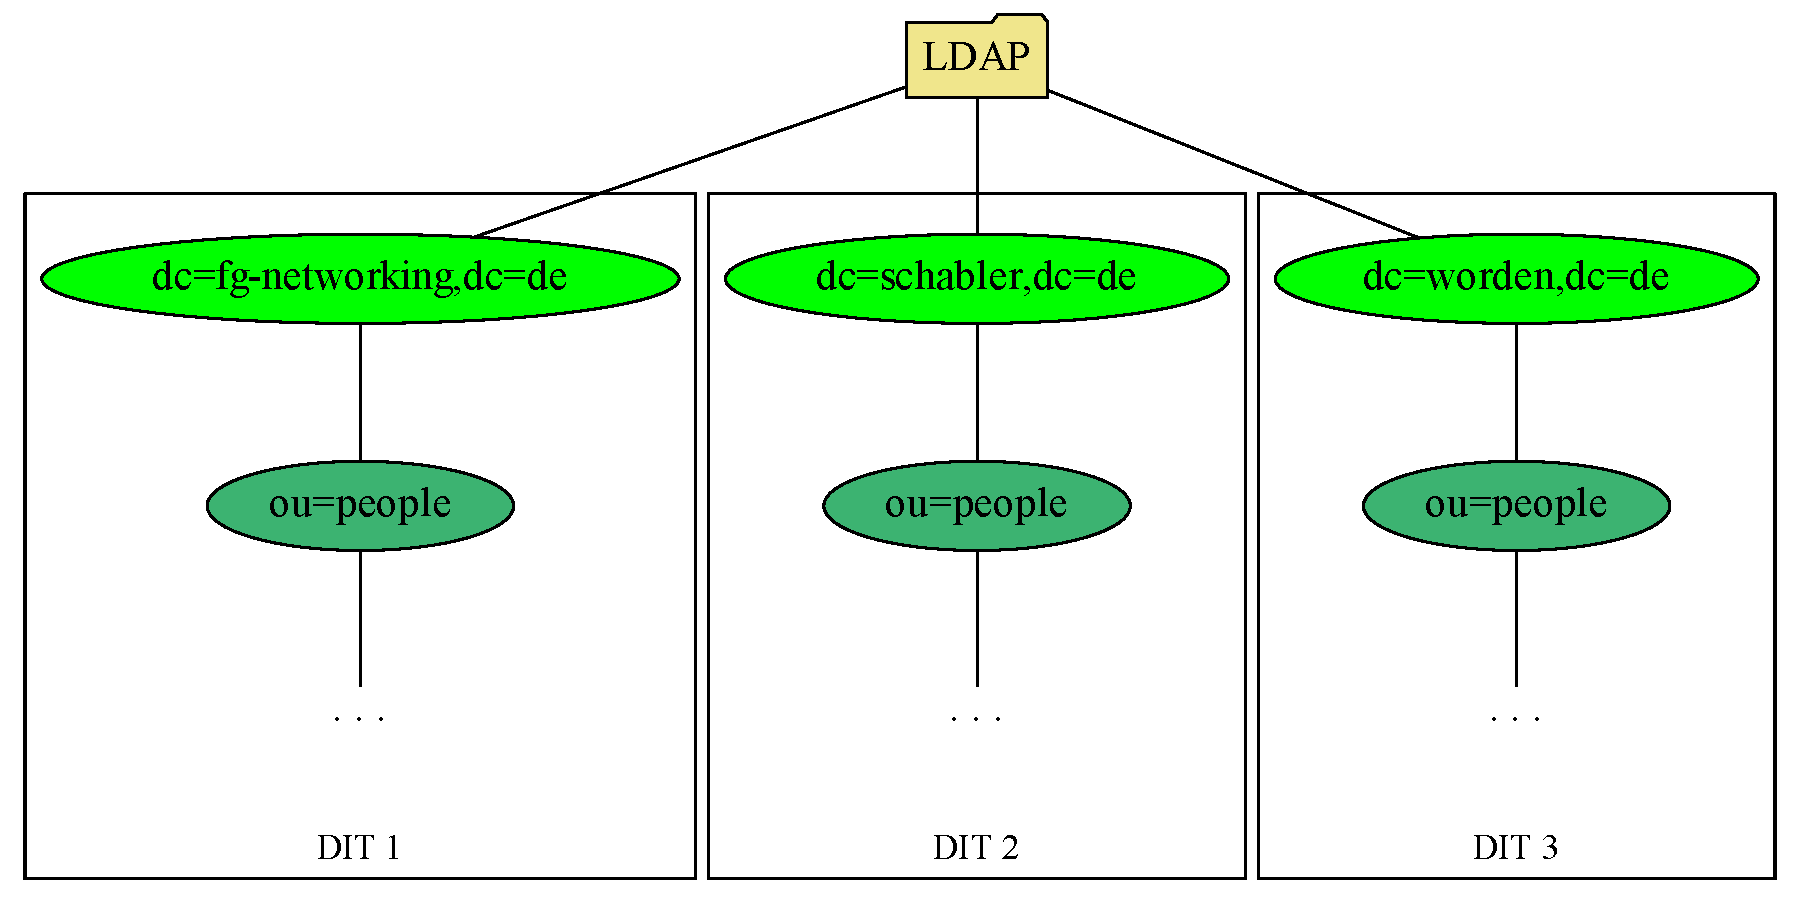
\includegraphics[width=0.95\textwidth]{Bilder/LDAP-fgn-planned.pdf}
\end{frame}


\begin{frame}{Realisierung des Ersatzservers (2)}
\begin{itemize}
	\item FreeRADIUS-Server mit Shared Secret für TU E-Mail-Server konfiguriert
	\item Anbindung an LDAP über mitgeliefertes Modul (Kommunikation über Loopback ohne SSL)
	\item Import von Anwenderkonten per generierter LDIF-Datei
	\item Einrichtung der Firewall
\end{itemize}
\end{frame}


\begin{frame}{Anbindung der Webservices etc}
LDAP wurde bereits ohne SSL von Apache, OpenVPN verwendet, deswegen kein große Umstellung:
\begin{itemize}
	\item geänderte Server-URL und BaseDN in Konfiguration von Apache und OpenVPN eintragen
	\item SSL-Zertifikat eintragen
\end{itemize}
Egroupware siehe Probleme
\end{frame}


\subsection{Qualitätssicherung}
\begin{frame}{Qualitätssicherung}
\begin{enumerate}
	\item Funktionstests:
	\begin{itemize}
		\item Webservices und OpenVPN wurden nach Umstellung getestet ob Login weiterhin möglich
		\item RADIUS Test mit \texttt{radtest} und Vergleich mit Antworten von CommuniGate-RADIUS (keine Praxistests möglich)
	\end{itemize}
	\item Sicherheitstests:
	\begin{itemize}
		\item Versuch von Anmelden mit falschen Anmeldeinformationen bei Webservices und OpenVPN
		\item Überprüfung OpenSSH-Server Konfiguration
		\item Port-Scan mit NMAP (aus fgn-Netz und extern)
	\end{itemize}
\end{enumerate}
\end{frame}


\subsection{Probleme und Lösungen}
\begin{frame}{Probleme und Lösungen}
\begin{enumerate}
	\item Design der LDAP-Baumstruktur
	\begin{itemize}
		\item ursprüngliche Idee eine Datenbank pro Domain, so erstellte Datenbanken ließen sich in der Praxis aber nicht ansprechen
		\item gelöst durch Umsetzung in einer Datenbank
	\end{itemize}
\end{enumerate}
\centering
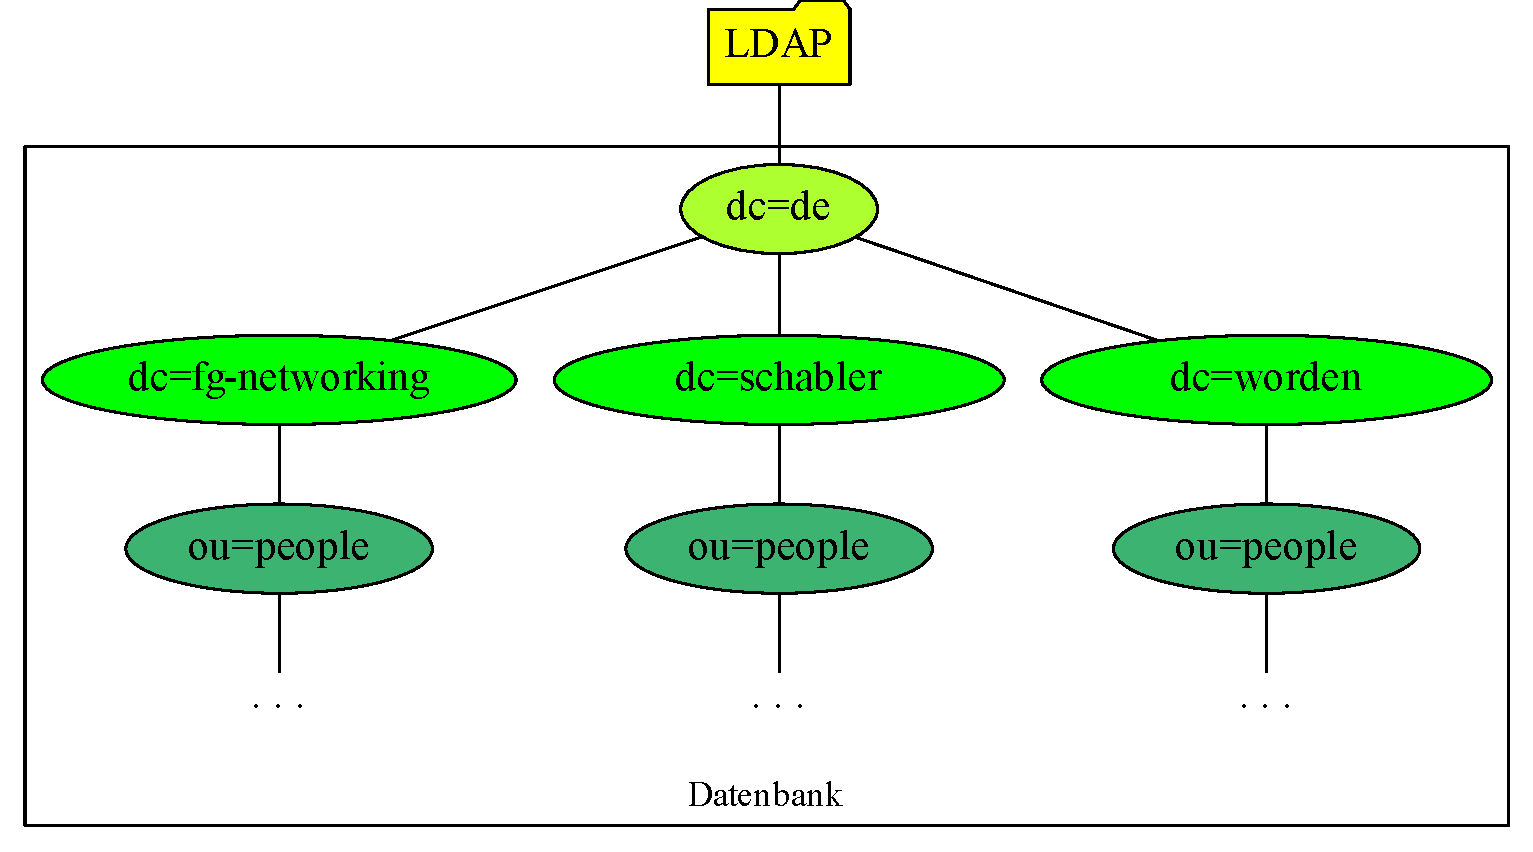
\includegraphics[width=0.79\textwidth]{Bilder/LDAP-fgn.pdf}
\end{frame}

\begin{frame}{Probleme und Lösungen (2)}
\begin{enumerate}
	\setcounter{enumi}{1}
	\item Egroupware
	\begin{itemize}
		\item fehlendes Passwort für Installer, Zuständiger in Urlaub
		\item Groupware sehr wichtig für Betrieb
		\item Umstellung verschoben, problemlos da alter Server weiterhin in Betrieb
	\end{itemize}
	\item neuer E-Mail-Server noch nicht fertig, deswegen manche Praxistests nicht möglich
	\begin{itemize}
		\item FreeRADIUS mit \texttt{radtest} getestet und Antwort mit CommuniGate verglichen
		\item Managed Switch probeweise an RADIUS angebunden
		\item Attribute für E-Mail-Integration nicht eingepflegt, entsprechend nicht getestet
	\end{itemize}
\end{enumerate}
\end{frame}


\section{Projektkosten}
\subsection{}
\begin{frame}{Projektkosten (mit Vergleich zu Alternative)}
\begin{table}
\centering
	\begin{tabularx}{0.8\textwidth}{|X|r|r|}
%		\hline
%		\mcc{4}{Kosten für die Einrichtung}\\
		\hline
		Kosten-	&	OpenLDAP \& &	CommuniGate-\\
		Kategorie	&	FreeRADIUS &	Upgrade\\
		\hline
		Hardware &	0,00\euro{} &	0,00\euro{}\\
		\hline
		Softwarelizenzen &	0,00\euro{} &	1.849,00\euro{}\\
		\hline
		Arbeitsaufwand &	2.485,00\euro{} &	2.485,00\euro{}\\
		\hhline{|=|=|=|}
		Gesamt &	2.485,00\euro{} &	4.334,00\euro{}\\
		\hline
	\end{tabularx}
\end{table}
\end{frame}


\section{Projektabschluss}
\subsection{Fazit}
\begin{frame}{Fazit}
\begin{itemize}
	\item alle Systeme außer Egroupware, E-Mail-Server umgestellt
	\item E-Mail-Server wird setzen neuer Attribute benötigen
	\item FreeRADIUS noch kein Praxistest
	\item Zeitplanung nicht optimal
	\begin{itemize}
		\item zu wenig Zeit für Design der Verzeichnisstruktur veranschlagt
		\item für die Vorbereitungen mehr Zeit eingeplant als benötigt
	\end{itemize}
\end{itemize}
\end{frame}


\subsection{Ausblick}
\begin{frame}{Ausblick}
	Erweiterungsmöglichkeiten
	\begin{enumerate}
		\item Anbindung neuer E-Mailserver (\texttt{postfix})
		\item Beschränkung des Nutzerkreises von Webtools
		\item Ersatz lokale Accounts
		\item Anbindung Managed Switches an FreeRADIUS
		\item Samba Domäne für Windows Rechner
	\end{enumerate}
\end{frame}


\section{} %section shall not be visible in navbar, hence empty name
\begin{frame}{Quellen}
	Vielen Dank für Ihre Aufmerksamkeit
	
	\medskip
	\medskip Diese Präsentation wurde mit \LaTeX{}-Beamer erstellt
	
	LDAP-Verzeichnisbaum Graphen erstellt mit GraphViz
\end{frame}


%\section{Projektkosten}
%\subsection{Projektkosten - Anschaffung}
%\begin{frame}{Projektkosten - Anschaffung}
%	\begin{tabularx}{\textwidth}{|X|r|r|r|}
%%		\hline
%%		\mcc{4}{Kosten für die Einrichtung}\\
%		\hline
%		Kosten-	&	OpenLDAP \& &	\centering CommuniGate- &	\\
%		Kategorie	&	FreeRADIUS &	\centering Upgrade &	Status Quo\\
%		\hline
%		Hardware &	0,00\euro{} &	0,00\euro{} &	0,00\euro{}\\
%		\hline
%		Softwarelizenzen &	0,00\euro{} &	1.849,00\euro{} &	0,00\euro{}\\
%		\hline
%		Arbeitsaufwand &	2.485,00\euro{} &	2.485,00\euro{} &	0,00\euro{}\\
%		\hhline{|=|=|=|=|}
%		Gesamt &	2.485,00\euro{} &	4.334,00\euro{} &	0,00\euro{}\\
%		\hline
%	\end{tabularx}
%\end{frame}


%\subsection{Projektkosten - Wartung}
%\begin{frame}{Projektkosten - Wartung}
%	\begin{tabularx}{\textwidth}{|X|r|r|r|}
%%		\hline
%%		\mcc{4}{Jährliche Kosten}\\
%		\hline
%		Kosten-	&	OpenLDAP \& &	CommuniGate- &	\\
%		Kategorie	&	FreeRADIUS &	Upgrade &	Status Quo\\
%		\hline
%		Hardware &	0,00\euro{} &	0,00\euro{} &	0,00\euro{}\\
%		\hline
%		Softwarelizenzen &	0,00\euro{} &	332,82\euro{} &	0,00\euro{}\\
%		\hline
%		Arbeitsaufwand &	355,00\euro{} &	213,00\euro{} &	2.350,00\euro{}\\
%		\hhline{|=|=|=|=|}
%		Gesamt &	355,00\euro{} &	545,82\euro{} &	2.350,00\euro{}\\
%		\hline
%	\end{tabularx}
%\end{frame}

\end{document}
